\section{Global Minimum Cut}
\label{sec:global}

Let~$G$ be undirected. We now turn our attention computing the global minimum cut of~$G$.
\note{TODO(kylejfox): Don't forget to give background for this problem and its difficulties in the introduction.}
To work with topology in computing a minimum cut, we use the following lemma which is similar very similar to Lemma~\ref{lem:cut-duality}.
We say a null-homologous even subgraph~$\eta$ is a \EMPH{separating subgraph} if it contains at least one edge.

\note{kylejfox: Throughout the dissertation I said vertex sets were cuts. We may need to reconcile with the $s,t$-cut papers.}
\begin{lemma}
\label{lem:mincut-z2}
Let~$G$ be an undirected graph with non-negative edge capacities, cellularly embedded on a surface~$\Sigma$ without boundary, let~$S$ be a minimum cut in~$G$, and let~$C$ be the edges crossing~$S$.  Then~$C^*$ is a minimum weight separating subgraph of~$G^*$.
\end{lemma}

\begin{proof}
  Let~$C$ be the edges crossing an arbitrary cut in~$G$.  The cut partitions the vertices of $G$
  into two disjoint subsets~$S$ and~$T$. Therefore, the dual subgraph~$C^*$
  partitions the faces of~$G^*$ into two disjoint subsets~$S^*$ and~$T^*$.
  Further,~$C^*$ is the boundary of the union of faces in~$S^*$, implying
  that~$C^*$ is null-homologous in~$\Sigma$ and therefore separating.

  Conversely, let~$C^*$ be an arbitrary separating subgraph of~$G^*$.
  As~$C^*$ is null-homologous, it is the boundary of a subset of the faces
  of~$G^*$.  Moreover, because $C^*$ is non-empty, it must be the boundary of
  a \emph{proper, non-empty} subset of faces.  Let $s^*$ and $t^*$ be faces
  of $G^*$ on either side of $C^*$.  Any path from~$s$ to~$t$ in the primal
  graph~$G$ must traverse at least one edge of~$C$.  We conclude that~$C$ crosses
  a cut (in particular, an $s,t$-cut).
\end{proof}

Fix an undirected graph~$G=(V,E)$, a non-negative weight function ${w\colon E\to \Real}$, and a cellular embedding of~$G$ on a surface~$\Sigma$ of genus~$g$ with at least two faces.  In light of Lemma \ref{lem:mincut-z2}, we focus our attention on finding a minimum weight separating subgraph of~$G$. 

Our algorithm separately considers two cases, illustrated in Figure~\ref{fig:global_cases}. Exactly one of these cases must apply to the minimum weight separating subgraph.
\begin{enumerate}
  \item
    Some minimum weight separating subgraph consists of a single contractible simple cycle.
  \item
    Every minimum weight separating subgraph can be decomposed into non-contractible simple cycles.
\end{enumerate}
%
\begin{figure}[h]
\centering
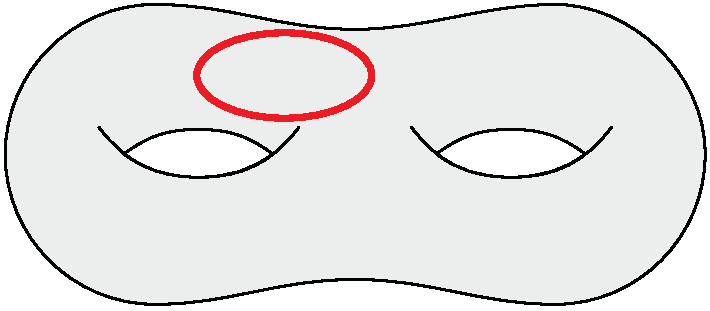
\includegraphics[height=1in]{Fig/shortcon2}\qquad
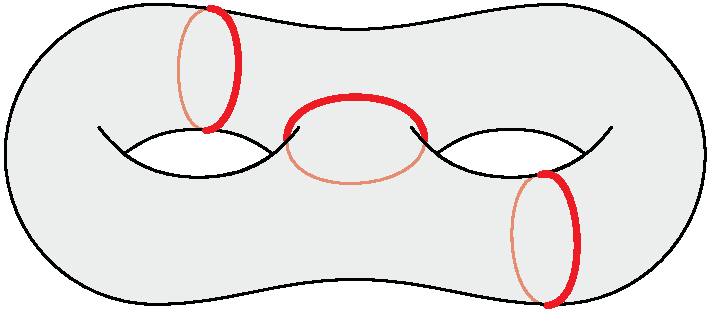
\includegraphics[height=1in]{Fig/homologous1}
\caption{Two types of minimum weight separating subgraphs: a contractible cycle and otherwise.}
\label{fig:global_cases}
\end{figure}
%

Throughout the rest of this section, we describe two subroutines to find minimum weight separating subgraphs that are designed with their corresponding condition in mind. If the corresponding condition does hold, the subroutine will return a separating subgraph with weight at most that of the minimum weight separating subgraph. Otherwise, the subroutine may return a higher weight separating subgraph. By running both subroutines and returning the best result, we find a minimum weight separating subgraph no matter which category it falls into.
